\documentclass[pdflatex,sn-nature]{sn-jnl}
\usepackage{amsmath,amssymb}
\usepackage{graphicx,booktabs,array,adjustbox}
\input{math_commands.tex}
\graphicspath{{figures/}}
\raggedbottom
\emergencystretch=2em

\begin{document}
\renewcommand{\arraystretch}{0.92}
\setlength{\tabcolsep}{4pt}

\setcounter{figure}{0}
\setcounter{table}{0}
\renewcommand{\thefigure}{S\arabic{figure}}
\renewcommand{\thetable}{S\arabic{table}}

\title{Supplementary Information for\\
FORGE decomposes RNA sequence recovery into memorisation, family transfer and
residual prediction error}

\date{}

\maketitle

\section*{Supplementary Note S1: AlphaFold 3 forward-folding control}

The forward-folding control evaluates whether the structure-to-sequence
information read by FORGE can be inverted by a contemporary folding model. The
four solved AI-designed pseudoknot constructs (PDB 10ZT, 10ZU, 11EH and 11AG;
design sequences embedded in a circularly permuted group II intron scaffold)
were submitted to the AlphaFold~3 server as the full deposited constructs,
matching the cryo-EM sample composition (11AG as a two-chain homodimer). Three
sequence classes were compared per construct: the true design sequence, the
FORGE-derived sequence (per-position maximum of the frozen-model readouts,
36.5--54.2\% identical to the true design) and the FORGE-derived sequence after
R-Net-guided reactivity refinement (48--59 mutations; reactivity profiles
optimised against the cryo-EM secondary structure with FORGE high-confidence
positions locked).

Evaluation used the designed segment (96--101 nt) after rigid-body fit to the
cryo-EM model. P-RMSD is the mean backbone-phosphate deviation; SS $F_1$ is the
$F_1$ of geometric Watson--Crick pairs (donor--acceptor distance
$\le$4.2~\AA); contact recovery is the fraction of cryo-EM inter-nucleotide
contacts ($<$7.5~\AA) reproduced. One AlphaFold~3 sample was retained per job; the archived batch summaries record a
single seed per job.

Only the true 10ZT sequence returned a near-experimental fold (6.6~\AA{}
P-RMSD, SS $F_1$ 0.99, 38/38 native pairs recovered). The remaining true
sequences failed at 14.1--26.9~\AA{} despite high secondary-structure recovery
(SS $F_1$ 0.69--0.88; register shifts within two base pairs recover 32--34 of
32--35 pairs), demonstrating secondary-structure recovery without
tertiary-geometry recovery. The FORGE-derived sequences were the worst input
class (SS $F_1 \le 0.13$ on three of four constructs), and R-Net-guided
refinement changed the AF3 outcome only marginally (SS $F_1$ 0.00--0.36; the
partial exception 11AG improved from 0.13 to 0.36 at 17.3~\AA{} P-RMSD).
Sequence recovery read out of geometry therefore does not invert to
AF3 consistency, with or without reactivity-guided sequence optimisation.

\begin{figure}[htbp]
\centering
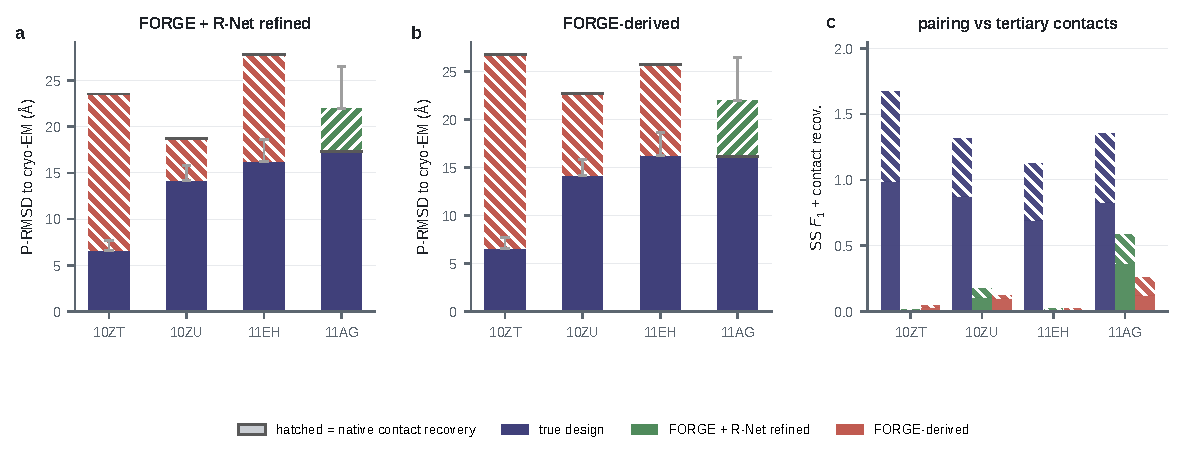
\includegraphics[width=\textwidth]{fig5_af3_combined.pdf}
\caption{\textbf{Forward-folding evaluation of the AI-designed pseudoknot
constructs (AlphaFold 3).} \textbf{a,} Delta P-RMSD of the FORGE-derived
sequence after R-Net-guided refinement relative to the true design sequence
(hatched segments: green, improvement; red, degradation; grey error bars,
range across archived server outputs for the true sequence; one sample per job). \textbf{b,} Same for the
FORGE-derived sequence. \textbf{c,} Watson--Crick pair recovery (SS $F_1$,
solid) and native tertiary contact recovery (hatched) for the three sequence
classes.}
\label{fig:af3_forward}
\end{figure}

\begin{figure}[htbp]
\centering
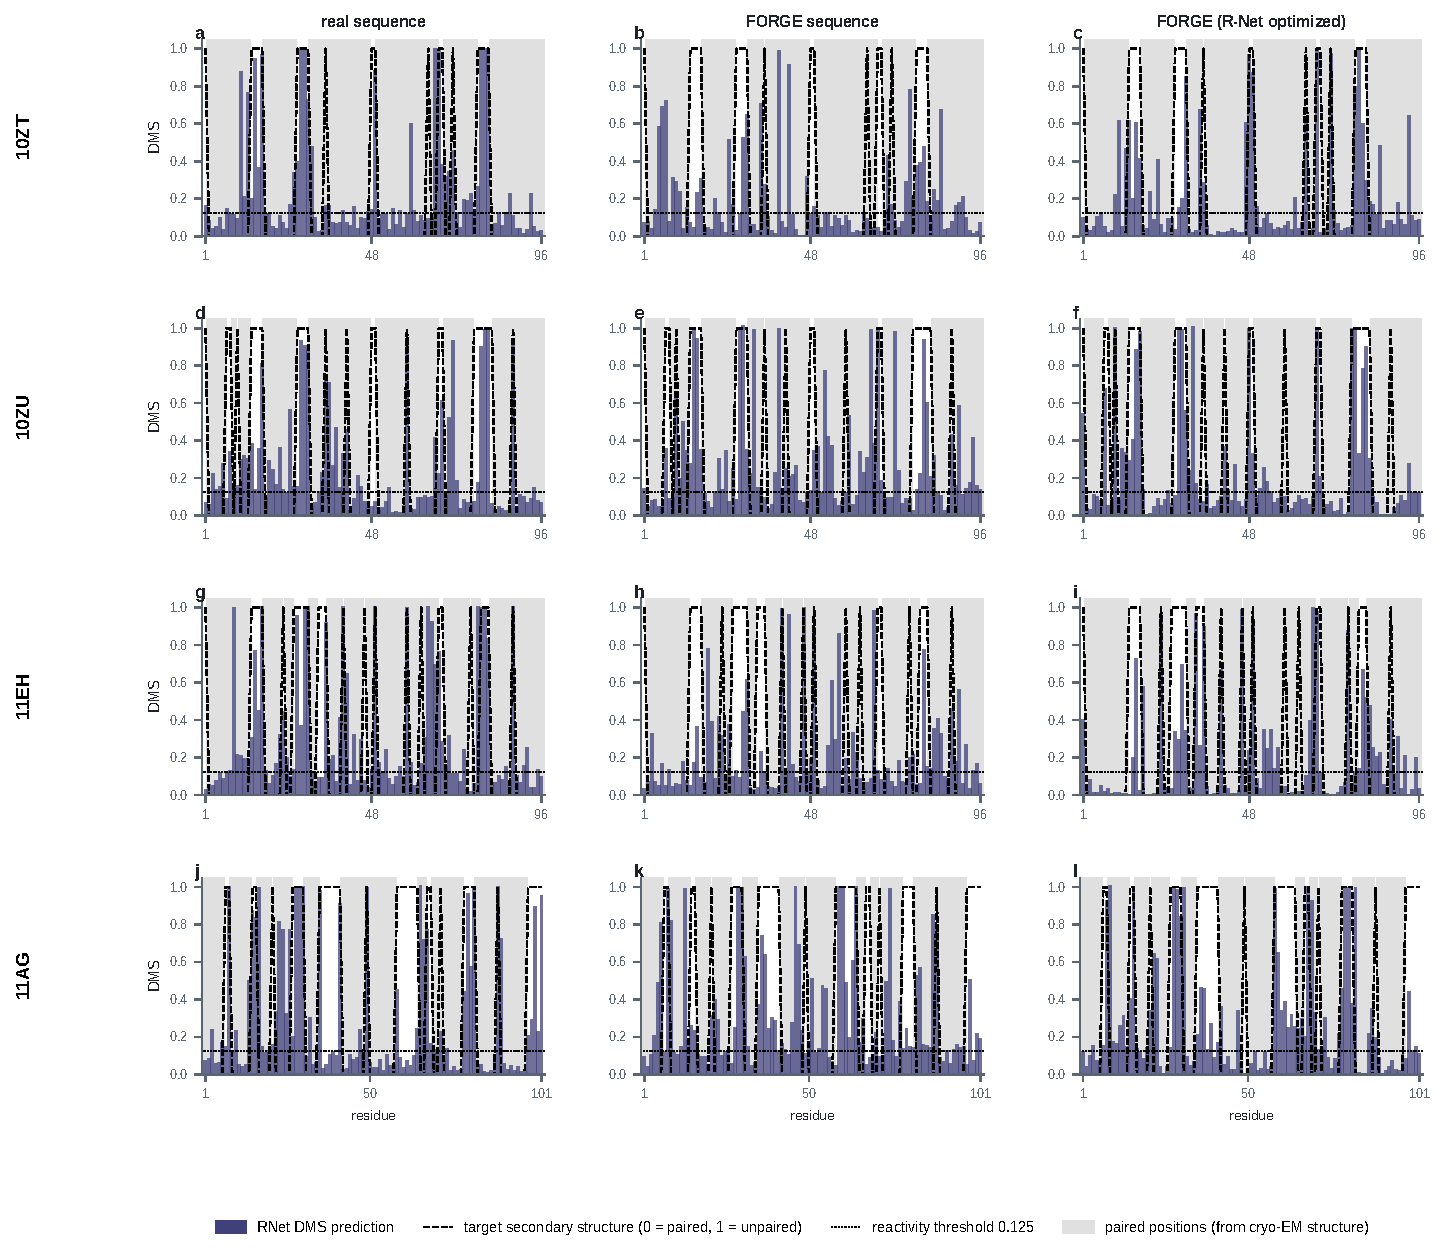
\includegraphics[width=\textwidth]{fig6_dms_target.pdf}
\caption{\textbf{R-Net reactivity predictions against the target secondary
structure.} Rows, PDB constructs; columns, sequence classes (true design,
FORGE-derived, FORGE-derived after R-Net refinement). Grey bands mark
positions paired in the cryo-EM structure; the dashed line is the binary
target profile (0, paired; 1, unpaired); the dotted line is the reactivity
threshold 0.125.}
\label{fig:dms_target}
\end{figure}

\clearpage
\begin{figure}[htbp]
\centering
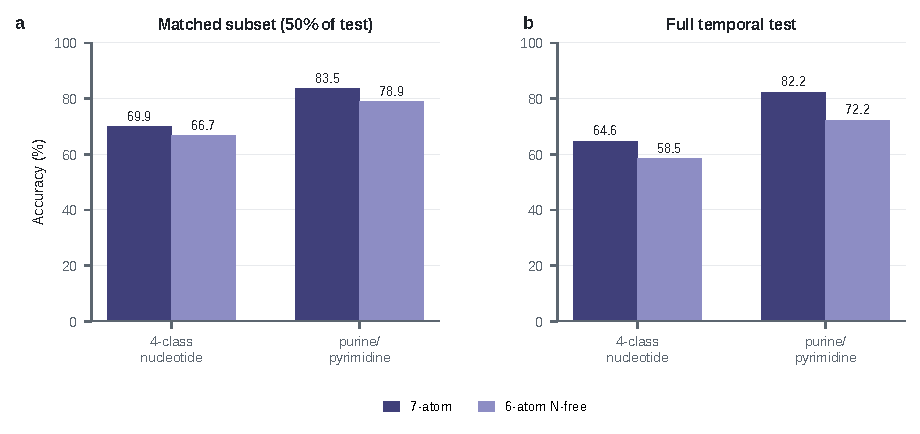
\includegraphics[width=\textwidth]{fig_s1_nfree.pdf}
\caption{\textbf{N-free retraining controls at both evaluation scales.}
\textbf{a,} Matched-subset retraining (200,000 training positions, 72,787 test
positions): the seven-atom model reached 69.9\% four-class recovery and 83.5\%
purine/pyrimidine accuracy, and the six-atom N-free model 66.7\% and 78.9\%.
\textbf{b,} Full temporal comparison: the seven-atom model on 4,135 chains
(291,331 positions) reached 64.6\% weighted recovery and 82.2\%
purine/pyrimidine accuracy; the N-free model on 4,167 chains (298,662 positions)
reached 58.5\% and 72.2\%. Both scales show that most
nucleotide-discriminating signal persists without the glycosidic nitrogen
coordinate.}
\label{fig:s_nfree}
\end{figure}

\begin{figure}[htbp]
\centering
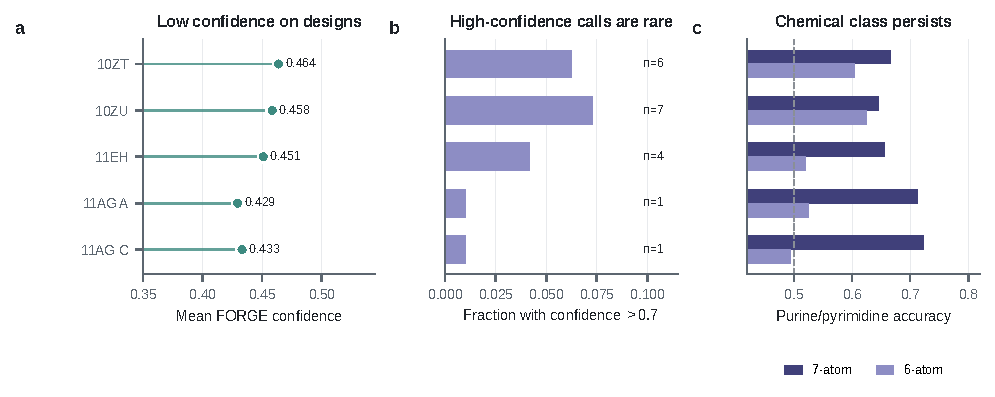
\includegraphics[width=\textwidth]{suppfig_stress_details.pdf}
\caption{\textbf{Confidence and chemical-class behaviour on the solved
AI-designed pseudoknots.} \textbf{a,} Mean per-position FORGE confidence per
chain (full post-2025 reference, 0.48). \textbf{b,} Fraction of positions with
confidence $>$0.7, annotated with the absolute number of high-confidence
positions. \textbf{c,} Purine/pyrimidine accuracy for the seven-atom and
six-atom N-free models (dashed line, random 50\%).}
\label{fig:s_stress}
\end{figure}

\begin{figure}[htbp]
\centering
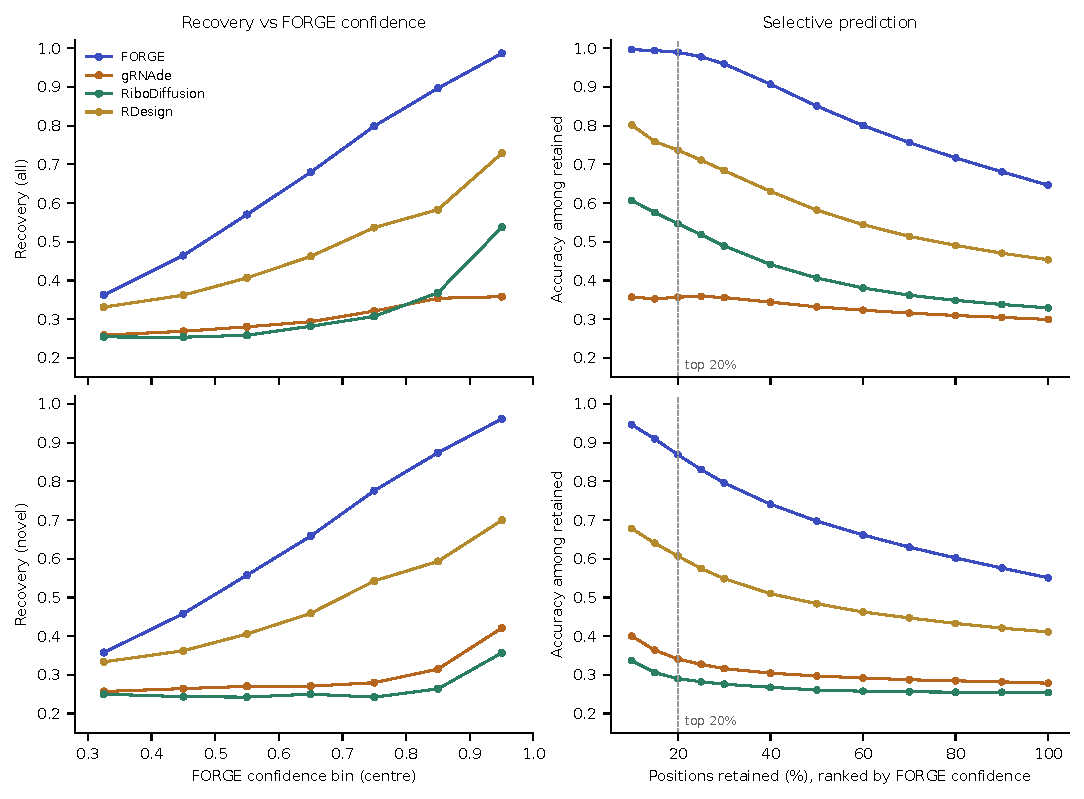
\includegraphics[width=\textwidth]{fig_s5_identifiability.pdf}
\caption{\textbf{Inverse-folding recovery tracks model-based predictability but falls far
below it.} Positions are ranked by FORGE confidence. \textbf{a,} Recovery across
confidence bins for FORGE and three public inverse-folding models on all post-2025
positions (top) and on sequence-novel positions only (bottom). \textbf{b,} Selective
prediction: accuracy on the retained top-$k$ fraction of positions. On sequence-novel
positions, the rank-defined top 20\% of sequence-novel positions (40,920 positions) are
recovered at 86.9\% by FORGE but only 60.7\% (RDesign), 34.1\% (gRNAde) and 29.0\%
(RiboDiffusion); this rank-defined subset is distinct from the confidence $\ge$0.9 bin
used in Supplementary Table S6. Values are computed
on the matched position mask; public models were not retrained on the FORGE split.}
\label{fig:s_identifiability}
\end{figure}

\section*{Supplementary Table S1: Evaluation subsets}

\begingroup\footnotesize
\begin{adjustbox}{width=\textwidth}
\begin{tabular}{p{0.20\textwidth}p{0.12\textwidth}p{0.14\textwidth}p{0.24\textwidth}p{0.14\textwidth}p{0.16\textwidth}}
\toprule
Analysis & Chains & Positions & Selection Criterion & Metric Type & Key Value \\
\midrule
Full post-2025 temporal & 4,135 & 291,331 & All post-2025 RNA chains & Weighted (micro) & 64.6\% [63.7, 65.6] \\
Full post-2025 temporal (per-chain) & 4,135 & 291,331 & All post-2025 RNA chains & Per-chain mean (macro) & 63.4\% \\
Exact-sequence repeat & 1,281 & 86,729 & Exact sequence in pre-2025 training & Weighted (micro) & 87.1\% [86.1, 88.2] \\
Sequence-novel & 2,854 & 204,602 & Exact sequence absent from training & Weighted (micro) & 55.1\% [54.3, 55.9] \\
Calibration (full) & 4,135 & 291,331 & All post-2025 RNA chains & ECE, 10 bins & 0.023 [0.020, 0.026] \\
In-domain reference & 591 & 53,288 & Sequence/PDB-disjoint held-out components & Weighted (micro) & 70.0\% \\
Temporal on same chains & 591 & 53,288 & Same held-out chains & Weighted (micro) & 54.0\% \\
Family-disjoint in-domain & 410 & 32,984 & Sequence/PDB/family-disjoint held-out components & Weighted (micro) & 50.4\% \\
Temporal on family-disjoint chains & 410 & 32,984 & Same family-disjoint chains & Weighted (micro) & 47.5\% \\
Cluster-disjoint temporal & 3,749 & 267,477 & No shared pre-2025 CD-HIT cluster & Weighted (micro) & 64.3\% [63.3, 65.3] \\
Novel and cluster-disjoint & 2,587 & 190,127 & Exact-novel and cluster-disjoint & Weighted (micro) & 55.2\% [54.4, 56.0] \\
Homology $<$80\% identity & 2,078 & 146,058 & Max identity to training $<$80\% & Weighted (micro) & 48.9\% \\
N-removed matched & 4,135 & 291,331 & Same positions as 7-atom & Weighted (micro) & 58.5\% [57.4, 59.6] \\
Stacking & 4,135 & 290,878 & Valid base-plane positions & Acc./AUC & 81.8\% / 0.879 \\
SS class & 2,138 & 163,395 & Exact DSSR-length chains & Acc./F1 & 78.5\% / 0.542 \\
Solvent exposure & 4,135 & 291,331 & Post-2025 chains with full-atom SASA labels & Pearson / $R^2$ & 0.948 / 0.899 \\
N-removed archived & 4,167 & 298,662 & Archived coverage & Weighted (micro) & 58.5\% \\
Native-vs-decoy & 50 & --- & 20--200 nt, baseline designs available & Chain-level AUROC & 0.41--1.00 by tier \\
Stress test & 5 chains & 490 & AI-designed pseudoknots, cryo-EM & Per-chain & 36.5--54.2\% \\
$k$-NN feature-space & 40 query & 1,134 & 10--200 nt, ref pool 80 chains & Position (micro) & $k$=10: 53.6\% \\
OpenKnot complete-case & 1,656 & --- & MFE F1 available & Design-level $\rho$ & $\rho_{\mathrm{partial}}$=+0.549 \\
\bottomrule
\end{tabular}
\end{adjustbox}
\endgroup

Calibration used 10 equal-width confidence bins from 0.25 to 1.0 on all 291,331
positions (ECE 0.023, Brier 0.304, negative log-likelihood 0.826; 500 chain-bootstrap
resamples). Per-chain abstention is right-censored at 90\% removal and unstable for
short chains; those estimates are descriptive only. A protein-proximal context analysis
was explored but is not reported as a result because chain-aware residue joins and
negative sampling were not independently validated. Synthetic tests confirmed that the Shrake--Rupley implementation reproduces the analytic
isolated-atom area and gives identical labels after a [100, 200, 300]~\AA{} translation.
A label-shuffle control trained on permuted SASA labels gave r = $-$0.011 (R$^2$ < 0),
confirming that the solvent-exposure signal is not an artifact of the regression pipeline.
The SASA readout uses the same cluster-permissive temporal test as the nucleotide readout
and is not a novelty-stratified estimate; residues with non-standard atom mappings are a
small minority and may carry noisier labels. Figure 2a uses matched-position
values (3,989/3,966/3,035 matched chains); the all-position published values
(30.1/33.5/46.4) are retained only for provenance and are not a controlled benchmark.

\section*{Supplementary Table S2: Stress-test chain homology verification}

\begingroup\footnotesize
\begin{adjustbox}{width=\textwidth}
\begin{tabular}{p{0.18\textwidth}p{0.08\textwidth}p{0.10\textwidth}p{0.12\textwidth}p{0.24\textwidth}p{0.14\textwidth}p{0.14\textwidth}}
\toprule
Chain & Length & In training? & Best seq.\ identity & Best match & PDB deposit & Download date \\
\midrule
10ZT (gRNAde) & 96 & No & 36.0\% & 5O9Z\_X\_2 (100 nt) & 2026-05-13 & 2026-05-24 \\
10ZU (MPNN-fixbb) & 96 & No & 38.5\% & 3ADC\_H\_C (88 nt) & 2026-05-13 & 2026-05-24 \\
11EH (Struct2Seq) & 96 & No & 34.4\% & 3A2K\_H\_C (77 nt) & 2026-05-14 & 2026-05-24 \\
11AG A (MPNN-RFdiff) & 101 & No & 35.6\% & 6CK4\_H\_D (101 nt) & 2026-05-14 & 2026-05-24 \\
11AG C (MPNN-RFdiff) & 101 & No & 35.6\% & 6CK4\_H\_D (101 nt) & 2026-05-14 & 2026-05-24 \\
\bottomrule
\end{tabular}
\end{adjustbox}
\endgroup

\clearpage
\section*{Supplementary Table S3: Multi-task label provenance and leakage control}

\begingroup\footnotesize
\begin{adjustbox}{width=\textwidth}
\begin{tabular}{p{0.16\textwidth}p{0.18\textwidth}p{0.32\textwidth}p{0.16\textwidth}p{0.18\textwidth}}
\toprule
Task & Label source & Forbidden inputs removed & Split & Baseline \\
\midrule
Nucleotide identity & PDB sequence & None; 7-atom coordinates only & Pre-2025 / post-2025 temporal & 25\% random \\
Base-pair state & DSSR dot-bracket & No DSSR, dot-bracket or pair labels used as features; all 935 descriptors computed from coordinates alone & Pre-2025 / post-2025 temporal & 63.1\% majority class \\
Reactivity target & RibonanzaNet inference & Sequence not used as input; backbone coordinates only & Pre-2025 / post-2025 temporal & Mean predictor \\
Solvent exposure & Full-atom Shrake--Rupley rSASA & Full-atom coordinates used only for labels; seven-atom input & Pre-2025 train / post-2025 test & Training median 0.395 \\
Stacking & Full-atom base-plane label & Sign-aligned normals; invalid planes masked & Pre-2025 train / post-2025 test & 6 \AA{}, 35$^\circ$, 3.5 \AA{} \\
SS class & DSSR dot-bracket & Exact length agreement; 3 classes & Pre-2025 train / post-2025 test & class-balanced weights \\
\bottomrule
\end{tabular}
\end{adjustbox}
\endgroup

\clearpage
\section*{Supplementary Table S4: Retrained atom-representation controls}

\begingroup\footnotesize
\begin{adjustbox}{width=\textwidth}
\begin{tabular}{p{0.26\textwidth}p{0.20\textwidth}p{0.10\textwidth}p{0.13\textwidth}p{0.20\textwidth}}
\toprule
Model & Atom channels used & Columns removed & Weighted recovery & $\Delta$ vs 7-atom (pp) \\
\midrule
7-atom control & P, O5$'$, C5$'$, C4$'$, C3$'$, O3$'$, N1/N9 & 0 & 61.94\% & --- \\
6-atom, N-neutralised & six; N-dependent features removed & 164 & 58.50\% & $-$3.43 [$-$3.65, $-$3.23] \\
6-atom, N at origin & six; N channel set to origin & 0 & 57.25\% & $-$4.69 [$-$4.97, $-$4.42] \\
6-atom, N = C4$'$ & six; dummy anchor & 0 & 57.42\% & $-$4.52 [$-$4.81, $-$4.24] \\
5-atom & O5$'$/O3$'$ features removed & 257 & 61.63\% & $-$0.31 [$-$0.47, $-$0.16] \\
3-atom & O5$'$/C5$'$/C3$'$/O3$'$ features removed & 435 & 61.04\% & $-$0.90 [$-$1.08, $-$0.71] \\
\bottomrule
\end{tabular}
\end{adjustbox}
\endgroup

\section*{Supplementary Table S5: Sequence-homology audit}

\begingroup\footnotesize
\begin{adjustbox}{width=\textwidth}
\begin{tabular}{p{0.18\textwidth}p{0.10\textwidth}p{0.14\textwidth}p{0.32\textwidth}p{0.20\textwidth}}
\toprule
Maximum identity to training & Chains & Positions & Definition & Weighted recovery \\
\midrule
$\geq$95\% & 1,580 & 112,697 & Best global identity $\geq$95\% & 85.0\% \\
90--95\% & 219 & 13,066 & Best identity 90--95\% & 67.4\% \\
80--90\% & 258 & 19,510 & Best identity 80--90\% & 62.8\% \\
$<$80\% & 2,078 & 146,058 & No training chain at $\geq$80\% identity & 48.9\% \\
\bottomrule
\end{tabular}
\end{adjustbox}
\endgroup

Identity is the maximum global Needleman--Wunsch identity to any pre-2025 training chain (edlib, 12-mer prefilter, 2,500-candidate cap; exact matches assigned 1.0).

\section*{Supplementary Table S6: Multi-learner convergence}

\begingroup\footnotesize
\begin{adjustbox}{width=\textwidth}
\begin{tabular}{p{0.20\textwidth}p{0.10\textwidth}p{0.11\textwidth}p{0.11\textwidth}p{0.11\textwidth}p{0.11\textwidth}}
\toprule
FORGE confidence & Positions & XGBoost & Logistic & MLP & $k$NN \\
\midrule
$<$0.5 & 118,156 & 41.7\% & 27.4\% & 31.8\% & 25.8\% \\
0.5--0.7 & 70,468 & 61.3\% & 33.1\% & 42.1\% & 32.9\% \\
0.7--0.8 & 19,941 & 79.9\% & 41.6\% & 60.5\% & 51.8\% \\
0.8--0.9 & 19,268 & 89.7\% & 48.5\% & 75.1\% & 66.6\% \\
$\geq$0.9 & 63,498 & 98.7\% & 64.3\% & 94.5\% & 91.5\% \\
\midrule
Overall & 291,331 & 64.6\% & 39.2\% & 52.8\% & 46.3\% \\
\bottomrule
\end{tabular}
\end{adjustbox}
\endgroup

Logistic regression (SGD, standardized), MLP (512--256, early stopping) and $k$NN ($k=10$) were trained on the same 200,000-position subsample; $k$NN was evaluated on a 20,000-position query subsample.

\section*{Supplementary Table S7: Frame-invariance audit}

\begingroup\footnotesize
\begin{adjustbox}{width=\textwidth}
\begin{tabular}{p{0.24\textwidth}p{0.18\textwidth}p{0.18\textwidth}p{0.28\textwidth}}
\toprule
Transform & Prediction agreement & Recovery & Note \\
\midrule
Original & --- & 59.3\% & 120 chains, 7,790 positions \\
Translation & 97.9\% & 59.5\% & translation-robust \\
Rotation & 59.0\% & 47.9\% & not rotation-invariant \\
Rigid (rotation + translation) & 58.2\% & 47.8\% & not rigid-invariant \\
Rotation-masked retrained model & 53.3\% & 62.1\% & 112 rotation-dependent features removed; \\
 & & & agreement under rotation remains low \\
Canonicalised-frame model & 99.6\% & 62.3\% & centred and principal-axis aligned before \\
 & & & featurization; repeats 84.7\%, exact-novel 52.8\%, \\
 & & & $<$80\% identity 47.0\%, ECE 0.012 \\
\bottomrule
\end{tabular}
\end{adjustbox}
\endgroup

The frame audit shows that the current pipeline is translation-robust but not rotation-invariant. A model retrained without the 112 rotation-dependent features retains 62.1\% unrotated recovery but only 53.3\% agreement under rotation, so it does not restore invariance. The canonicalised-frame model (62.3\% recovery, 99.6\% agreement) reproduces the decomposition (84.7\% repeats, 52.8\% exact-novel, 47.0\% below 80\% identity; ECE 0.012) with a paired cost of 2.35~pp, so the main conclusions are frame-safe at a small cost; the headline estimates themselves apply to the locked coordinate convention.



\section*{Supplementary Table S8: within-family method and resolution strata}

\begingroup\footnotesize
\begin{adjustbox}{width=\textwidth}
\begin{tabular}{llrrrr}
\toprule
Family & Method & Resolution (\AA) & Chains & Positions & Recovery \\
\midrule
tRNA & cryo-EM & <=2.5 & 101 & 7,525 & 79.7\% \\
tRNA & cryo-EM & 2.5-3.0 & 178 & 13,327 & 71.7\% \\
tRNA & cryo-EM & 3.0-3.5 & 95 & 7,031 & 70.1\% \\
tRNA & cryo-EM & >3.5 & 84 & 6,372 & 83.0\% \\
tRNA & X-ray & <=2.5 & 37 & 2,717 & 86.5\% \\
tRNA & X-ray & 2.5-3.0 & 44 & 3,253 & 77.2\% \\
tRNA & X-ray & 3.0-3.5 & 1 & 88 & 73.9\% \\
5S\_rRNA & cryo-EM & <=2.5 & 85 & 10,106 & 86.2\% \\
5S\_rRNA & cryo-EM & 2.5-3.0 & 126 & 14,979 & 84.9\% \\
5S\_rRNA & cryo-EM & 3.0-3.5 & 71 & 8,440 & 87.7\% \\
5S\_rRNA & cryo-EM & >3.5 & 51 & 6,125 & 92.8\% \\
5S\_rRNA & X-ray & <=2.5 & 10 & 1,200 & 100.0\% \\
5S\_rRNA & X-ray & 2.5-3.0 & 22 & 2,644 & 100.0\% \\
5\_8S\_rRNA & cryo-EM & <=2.5 & 33 & 5,148 & 90.2\% \\
5\_8S\_rRNA & cryo-EM & 2.5-3.0 & 70 & 10,775 & 95.3\% \\
5\_8S\_rRNA & cryo-EM & 3.0-3.5 & 27 & 4,165 & 95.7\% \\
5\_8S\_rRNA & cryo-EM & >3.5 & 12 & 1,865 & 97.8\% \\
Purine & cryo-EM & 2.5-3.0 & 5 & 703 & 43.7\% \\
Purine & X-ray & <=2.5 & 5 & 346 & 40.5\% \\
Purine & X-ray & 2.5-3.0 & 9 & 637 & 37.0\% \\
Purine & X-ray & 3.0-3.5 & 3 & 211 & 34.1\% \\
RNaseP\_bact\_b & cryo-EM & 2.5-3.0 & 42 & 17,514 & 50.7\% \\
RNaseP\_bact\_b & cryo-EM & 3.0-3.5 & 34 & 14,178 & 51.3\% \\
RNaseP\_bact\_b & cryo-EM & >3.5 & 2 & 834 & 48.6\% \\
AdoCbl-II & X-ray & <=2.5 & 24 & 1,800 & 61.8\% \\
AdoCbl-II & X-ray & 2.5-3.0 & 5 & 376 & 63.3\% \\
\bottomrule
\end{tabular}
\end{adjustbox}
\endgroup

Within-family strata are descriptive; families with fewer than five chains in a bin are
omitted. The non-monotonic pattern (for example, cryo-EM tRNA chains above 3.5~\AA{}
recover better than 3.0--3.5~\AA{} chains) is consistent with family and length
confounding and is why the adjusted model, not the raw bins, is used for inference.

\clearpage
\section*{Supplementary Figure S6: design-objective separability and stress tests}

\begin{figure}[htbp]
\centering
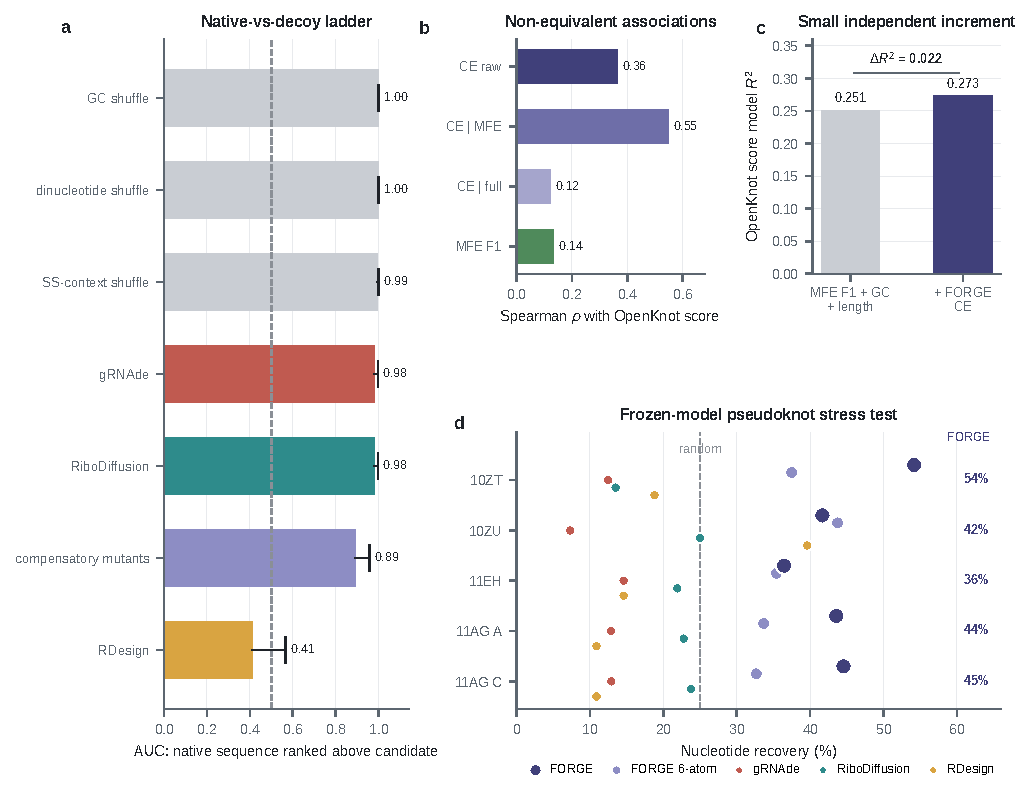
\includegraphics[width=\textwidth]{fig6_design_stress.pdf}
\caption{\textbf{Design-objective separability and frozen-model stress tests.}
\textbf{a,} Native-versus-decoy AUC ladder across composition-preserving
shuffles, learned inverse-folding outputs, compensatory pair swaps and RDesign
outputs (error bars, Wilson 95\% intervals from stored tier aggregates; dashed
line, no native preference). \textbf{b,} Raw and partial Spearman associations
between FORGE cross-entropy, RNAfold MFE F1 and OpenKnot experimental score in
the complete-case design subset ($n=1,656$). \textbf{c,} Linear-model fit to
OpenKnot score before and after adding FORGE cross-entropy to MFE F1, GC
content and length ($\Delta R^2=0.022$, $p=4.3\times10^{-12}$). \textbf{d,}
Per-chain nucleotide recovery (dot plot) for FORGE, the six-atom N-free
retrained model and public pretrained baselines on five solved AI-designed
pseudoknot chains; the dashed line marks random recovery.}
\label{fig:s_design}
\end{figure}

\clearpage
\section*{Supplementary Figure S7: representation controls and feature-space ambiguity}

\begin{figure}[htbp]
\centering
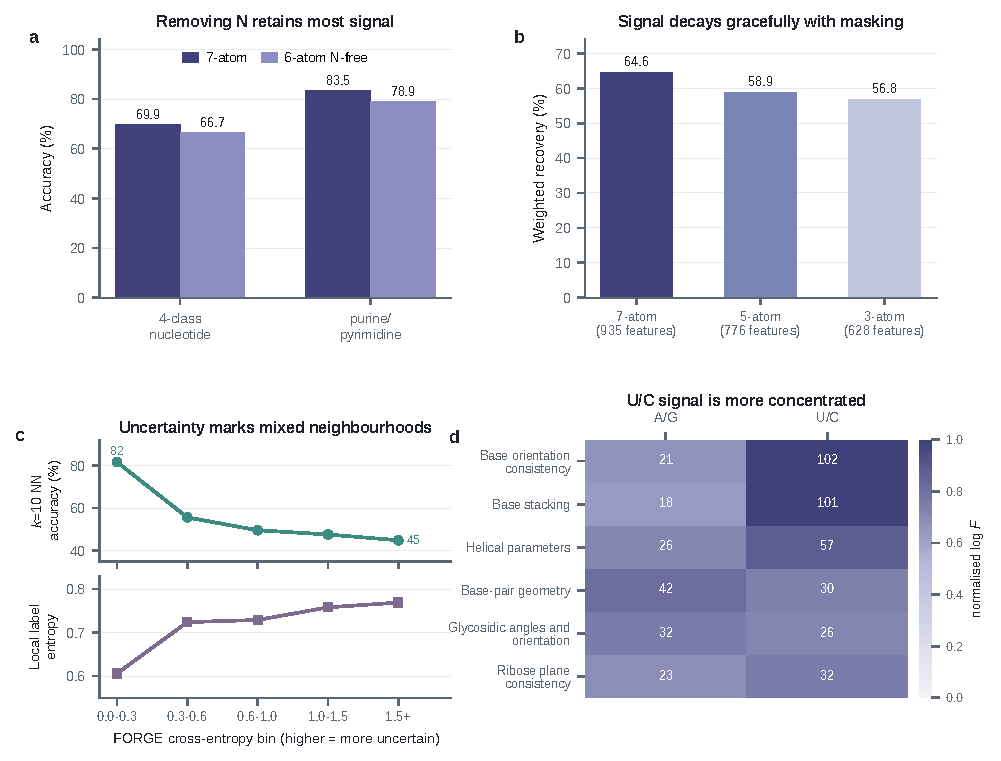
\includegraphics[width=\textwidth]{fig3_representation_controls.pdf}
\caption{\textbf{Representation controls and feature-space ambiguity.}
\textbf{a,} Matched-subset retraining after N-channel neutralisation (4-class recovery
and purine/pyrimidine accuracy; full comparison 64.6\% versus 58.5\%). \textbf{b,}
Inference-time atom-feature masking on the full post-2025 set (7-, 5- and 3-atom masks
with the number of retained features). \textbf{c,} Leave-one-chain-out $k=10$
nearest-neighbour accuracy (top) and local label entropy (bottom) across FORGE
cross-entropy bins. \textbf{d,} Feature-ontology categories with the strongest
discrimination for the A/G and U/C ambiguous pairs (colour, normalised log-transformed
ANOVA $F$-statistic; numbers, raw $F$).}
\label{fig:s_controls}
\end{figure}

\section*{Supplementary Methods: retrospective strata and feature attribution}

\paragraph{Structure metadata.} Resolution and experimental method were retrieved for
all 1,517 distinct post-2025 PDB entries from the RCSB entry API on 2026-10-30
(\texttt{pdb\_metadata.json}). Resolution was taken from the first value of
\texttt{resolution\_combined}; entries without a numeric resolution were kept in an
explicit missing/NMR category for descriptive strata and were excluded from the adjusted
OLS model. X-ray and cryo-EM resolutions were binned separately and never pooled without
method adjustment.

\paragraph{Adjusted model.} Chain-level recovery was modelled as
\texttt{recovery \textasciitilde{} log(length) + method + resolution + family +
release year + novelty} by OLS with PDB-clustered standard errors, using the 4,084
chains with numeric resolution (51 missing-resolution chains excluded). The resolution coefficient was $+1.1$~pp per \AA{}
(95\% CI $-0.2$ to $+2.5$; $p=0.10$) and the X-ray-versus-cryo-EM term was $+1.8$~pp
($p=0.26$); exact-novel, cluster-disjoint chains recovered 17.7~pp less ($p<10^{-24}$)
and 2026 entries 6.3~pp more than 2025 entries ($p<10^{-5}$). The outcome is bounded in
[0,1]; OLS coefficients are associational and may be attenuated. Family terms used the six groups with at least 50 chains; smaller families were pooled as
``other''. The descriptive family panel uses families with at least 20 chains. These estimates are association-only and do not
identify causal quality effects.

\paragraph{Grouped permutation importance.} The 935 descriptors were mapped to the six
feature-ontology categories (914 mapped; 21 unclassified). For each task and category,
all columns in the category were permuted with a common row permutation, preserving
within-category correlations, on a fixed 20,000-position post-2025 sample; the metric
drop was averaged over five fixed-seed permutations. Nucleotide identity used accuracy, base-pair state AUC and solvent accessibility Pearson $r$ (not $R^2$). Point estimates are mean per-chain drops; 95\% intervals are chain bootstrap (2,000 resamples); five fixed permutations; absolute drops and the five-permutation range are exploratory and conditional on the frozen model, and are in the source CSV. The frozen models were not retrained. Groups differ substantially in size (14--693 features); drops are group-level and are not normalised per feature.

\paragraph{SASA ablation controls.} The solvent-accessibility regressor was retrained
on the same 200,000-position pre-2025 sample after setting to zero the four explicit
\texttt{sasa\_*} features, the 24 global/centre descriptors, the nine local-density
features, or all three groups (35 features). Pearson $r$ fell from 0.948 (all features)
to 0.948 (no explicit SASA), 0.942 (no SASA + global) and 0.942 (no SASA + global +
density), showing that the signal is distributed across local geometry rather than carried by a single proxy. Zeroing is an ablation, not physical feature removal; it supports packing-associated coordinate predictability, not independent chemistry.

\paragraph{Case-study selection.} Selection rules were documented before chain-level outcomes were inspected; A is a confidence-selected positive control and B is family-targeted:
(A) lexicographically first X-ray chain at $\leq2.0$~\AA{} or cryo-EM chain at
$\leq3.0$~\AA{}, length 50--300~nt, at least 30\% of positions at confidence $\geq0.9$,
family in 5S rRNA, 5.8S rRNA or tRNA; (B) lexicographically first Purine or K10\_TLS
chain, length 50--300~nt; (C) lexicographically first post-2025 chain with at least 10
DSSR pseudoknot positions and length 50--300~nt; (D) the median-length chain among the
first 100 lexicographic exact-novel, cluster-disjoint chains. Full eligible lists (425/22/146/100 chains for A--D) and selected IDs are archived in \texttt{case\_selection\_full.json}. Rule A is a confidence-selected positive control; Rule B is family-targeted (Purine/K10\_TLS, known at the family level to be low-recovery); Rules C/D are outcome-blind. 10ZT/10ZU/11EH/11AG are not in the locked post-2025 feature set, so Rule C uses a DSSR pseudoknot chain. These provenance details are descriptive and do not support statistical inference.



\section*{Supplementary Table S9: complete multiplicity table}

\begingroup\scriptsize
\begin{adjustbox}{width=\textwidth}
\begin{tabular}{llllll}
\toprule
Analysis family & Test & Estimate & $p$ & BH $q$ & Status \\
\midrule
Family & 5.8S\_rRNA & +33.9 pp & $8.5\times10^{-131}$ & $3.4\times10^{-130}$ & adjusted \\
Family & 5S\_rRNA & +24.9 pp & $9.9\times10^{-76}$ & $2.0\times10^{-75}$ & adjusted \\
Family & RNaseP & +1.0 pp & 0.496 & 0.496 & adjusted \\
Family & tRNA & +18.6 pp & $9.2\times10^{-63}$ & $1.2\times10^{-62}$ & adjusted \\
Length & <50 & +0.4 pp & 0.759 & 0.759 & adjusted \\
Length & 50-100 & +0.5 pp & 0.732 & 0.759 & adjusted \\
Length & 201-500 & -1.8 pp & 0.430 & 0.759 & adjusted \\
Resolution & <=2.0 & -6.0 pp & 0.059 & 0.149 & adjusted \\
Resolution & 2.0-2.5 & +3.4 pp & 0.147 & 0.244 & adjusted \\
Resolution & 3.0-3.5 & -0.2 pp & 0.911 & 0.911 & adjusted \\
Resolution & 3.5-4.0 & +1.7 pp & 0.506 & 0.633 & adjusted \\
Resolution & >4.0 & +5.4 pp & $7.1\times10^{-4}$ & 0.004 & adjusted \\
Feature group & Intra-nt backbone (nucleotide) & 20.4\% & $1.0\times10^{-6}$ & $1.4\times10^{-6}$ & exploratory \\
Feature group & Global/centre (nucleotide) & 2.2\% & $1.0\times10^{-6}$ & $1.4\times10^{-6}$ & exploratory \\
Feature group & Unclassified (nucleotide) & 7.9\% & $1.0\times10^{-6}$ & $1.4\times10^{-6}$ & exploratory \\
Feature group & Helical/torsion (nucleotide) & 2.0\% & $1.0\times10^{-6}$ & $1.4\times10^{-6}$ & exploratory \\
Feature group & Local neighborhood (nucleotide) & 1.4\% & 0.002 & 0.002 & exploratory \\
Feature group & Glycosidic (nucleotide) & 2.0\% & $1.0\times10^{-6}$ & $1.4\times10^{-6}$ & exploratory \\
Feature group & Inter-nt edge (nucleotide) & 30.6\% & $1.0\times10^{-6}$ & $1.4\times10^{-6}$ & exploratory \\
Feature group & Intra-nt backbone (basepair) & 0.1\% & 0.557 & 0.561 & exploratory \\
Feature group & Global/centre (basepair) & 2.4\% & $1.0\times10^{-6}$ & $1.4\times10^{-6}$ & exploratory \\
Feature group & Unclassified (basepair) & 0.1\% & 0.145 & 0.160 & exploratory \\
Feature group & Helical/torsion (basepair) & -0.1\% & 0.561 & 0.561 & exploratory \\
Feature group & Local neighborhood (basepair) & 0.3\% & 0.144 & 0.160 & exploratory \\
Feature group & Glycosidic (basepair) & 0.4\% & $1.0\times10^{-6}$ & $1.4\times10^{-6}$ & exploratory \\
Feature group & Inter-nt edge (basepair) & 23.9\% & $1.0\times10^{-6}$ & $1.4\times10^{-6}$ & exploratory \\
Feature group & Intra-nt backbone (sasa) & 3.9\% & $1.0\times10^{-6}$ & $1.4\times10^{-6}$ & exploratory \\
Feature group & Global/centre (sasa) & 31.5\% & $1.0\times10^{-6}$ & $1.4\times10^{-6}$ & exploratory \\
Feature group & Unclassified (sasa) & 0.4\% & 0.002 & 0.002 & exploratory \\
Feature group & Helical/torsion (sasa) & 2.1\% & $1.0\times10^{-6}$ & $1.4\times10^{-6}$ & exploratory \\
Feature group & Local neighborhood (sasa) & 10.0\% & $1.0\times10^{-6}$ & $1.4\times10^{-6}$ & exploratory \\
Feature group & Glycosidic (sasa) & 2.4\% & $1.0\times10^{-6}$ & $1.4\times10^{-6}$ & exploratory \\
Feature group & Inter-nt edge (sasa) & 12.2\% & $1.0\times10^{-6}$ & $1.4\times10^{-6}$ & exploratory \\
Covariate & novelty & -- & $2.6\times10^{-25}$ & $5.3\times10^{-25}$ & adjusted \\
Covariate & year\_2026\_vs\_2025 & -- & $9.7\times10^{-6}$ & $9.7\times10^{-6}$ & adjusted \\
SASA threshold & threshold 0.3 & AUC 0.971 & -- & -- & descriptive \\
SASA threshold & threshold 0.35 & AUC 0.946 & -- & -- & descriptive \\
SASA threshold & threshold 0.4 & AUC 0.940 & -- & -- & descriptive \\
SASA threshold & threshold 0.45 & AUC 0.979 & -- & -- & descriptive \\
SASA threshold & threshold 0.5 & AUC 0.980 & -- & -- & descriptive \\
SASA threshold & threshold 0.55 & AUC 0.990 & -- & -- & descriptive \\
SASA threshold & threshold 0.6 & AUC 0.993 & -- & -- & descriptive \\
\bottomrule
\end{tabular}
\end{adjustbox}
\endgroup

$p$-values for family, resolution and length contrasts come from PDB-clustered OLS with
the other strata as covariates; feature-group $p$-values are two-sided chain-bootstrap
values; covariates are the novelty and 2026-vs-2025 terms. BH correction is applied
within each declared family. SASA thresholds are descriptive and carry no $p$-value. Feature-group $p$-values are bootstrap sign probabilities after five permutations (floor $10^{-6}$) and are exploratory, not permutation-null tests. The five sensitivity terms are corrected separately in Table S10b.

\section*{Supplementary Table S10: model sensitivity and importance controls}

\begingroup\scriptsize
\begin{adjustbox}{width=\textwidth}
\begin{tabular}{lrr}
\toprule
Resolution sensitivity & Estimate & $p$ \\
\midrule
Linear resolution (pp/\AA) & +1.13 & 0.099 \\
Logit OLS (logit/\AA) & +0.143 & 0.119 \\
Fractional logit (logit/\AA) & +0.054 & 0.107 \\
X-ray only (pp/\AA) & +4.54 & 0.016 \\
Spline joint test & -- & $2.8\times10^{-4}$ \\
Quadratic term & -- & 0.830 \\
Method x resolution & -- & 0.119 \\
Family x resolution & -- & 0.017 \\
\bottomrule
\end{tabular}
\end{adjustbox}
\endgroup

Missing resolution: 51 chains (mean recovery 45.5\%); included $n=4{,}084$, of which
1{,}411 carry an Rfam label. Maximum Cook's distance 0.0053; maximum VIF 4.83; 1,472 PDB clusters. Grouped SHAP uses 5,000 positions per task; group sizes 14--693 and shares sum to 100\%.

\begingroup\scriptsize
\begin{adjustbox}{width=\textwidth}
\begin{tabular}{lrrr}
\toprule
Leave-one-group-out (pp change) & Nucleotide & Base-pair & SASA \\
\midrule
Intra-nt backbone & +2.20 & +0.11 & -0.01 \\
Global/centre & +0.39 & +0.33 & +0.57 \\
Unclassified & -0.24 & +0.02 & -0.04 \\
Helical/torsion & -0.43 & +0.10 & +0.04 \\
Local neighborhood & -0.28 & +0.04 & +0.06 \\
Glycosidic & +0.02 & +0.08 & +0.09 \\
Inter-nt edge & +1.65 & +0.89 & +0.87 \\
\bottomrule
\end{tabular}
\end{adjustbox}
\endgroup

Label-shuffle controls (training labels permuted): nucleotide accuracy 26.2\% (chance
25\%), base-pair AUC 0.502 (chance 0.5), SASA Pearson $r=-0.011$ (chance 0). These are pipeline sanity checks; they do not test train/test homology or coordinate shortcuts, which are covered by the temporal/cluster audits. A single shuffle seed is a chance-level control, not a calibrated null.

\begingroup\scriptsize
\begin{adjustbox}{width=\textwidth}
\begin{tabular}{lrrr}
\toprule
Grouped SHAP share (\%) & Nucleotide & Base-pair & SASA \\
\midrule
Intra-nt backbone & 18.8 & 6.6 & 9.3 \\
Global/centre & 5.3 & 12.4 & 27.9 \\
Unclassified & 6.0 & 4.4 & 1.7 \\
Helical/torsion & 5.9 & 6.0 & 3.7 \\
Local neighborhood & 7.4 & 7.8 & 15.5 \\
Glycosidic & 3.7 & 4.1 & 3.3 \\
Inter-nt edge & 52.8 & 58.8 & 38.7 \\
\bottomrule
\end{tabular}
\end{adjustbox}
\endgroup

\section*{Supplementary Table S10b: exploratory sensitivity terms}

\begingroup\scriptsize
\begin{adjustbox}{width=\textwidth}
\begin{tabular}{lrrr}
\toprule
Sensitivity term & Estimate & $p$ & BH $q$ \\
\midrule
Spline joint test & -- & $2.8\times10^{-4}$ & 0.0014 \\
X-ray-only resolution & $+4.54$ pp/\AA & 0.016 & 0.028 \\
Quadratic resolution & -- & 0.830 & 0.830 \\
Method $\times$ resolution & -- & 0.119 & 0.149 \\
Family $\times$ resolution & -- & 0.017 & 0.028 \\
\bottomrule
\end{tabular}
\end{adjustbox}
\endgroup

BH correction is across these five exploratory sensitivity terms and does not replace
the primary strata contrasts in Table S9. X-ray-only is the resolution slope within
X-ray chains; the adjusted X-ray-versus-cryo-EM method term (+1.8 pp) is a distinct
estimand from the main model.

\section*{Supplementary Table S11: SASA threshold and novelty sensitivity}

\begingroup\scriptsize
\begin{adjustbox}{width=\textwidth}
\begin{tabular}{rrrr}
\toprule
Exposure threshold & Exposed fraction & AUC & Average precision \\
\midrule
0.3 & 0.834 & 0.971 & 0.993 \\
0.35 & 0.690 & 0.946 & 0.973 \\
0.4 & 0.424 & 0.940 & 0.933 \\
0.45 & 0.270 & 0.979 & 0.954 \\
0.5 & 0.173 & 0.980 & 0.925 \\
0.55 & 0.110 & 0.990 & 0.947 \\
0.6 & 0.077 & 0.993 & 0.938 \\
\bottomrule
\end{tabular}
\end{adjustbox}
\endgroup

\begingroup\scriptsize
\begin{adjustbox}{width=\textwidth}
\begin{tabular}{lrrrr}
\toprule
Population & Chains & Positions & Length-weighted mean per-chain $r$ & 95\% CI \\
\midrule
All & 4,135 & 291,331 & 0.922 & [0.920, 0.924] \\
Exact repeat & 1,281 & 86,729 & 0.954 & [0.951, 0.957] \\
Exact novel & 2,854 & 204,602 & 0.909 & [0.906, 0.911] \\
<80\% identity & 2,078 & 146,058 & 0.903 & [0.901, 0.905] \\
Novel + cluster-disjoint & 2,587 & 190,127 & 0.910 & [0.908, 0.912] \\
\bottomrule
\end{tabular}
\end{adjustbox}
\endgroup

AUC remains high (0.940--0.993) but is threshold-dependent; the novelty values are
length-weighted means of per-chain $r$, not the pooled $r=0.948$. SASA remains a
coordinate-derived packing proxy on the cluster-permissive temporal population.

\section*{Supplementary Figure S12: complementary descriptor and stratum panels}

\begin{figure}[htbp]
\centering
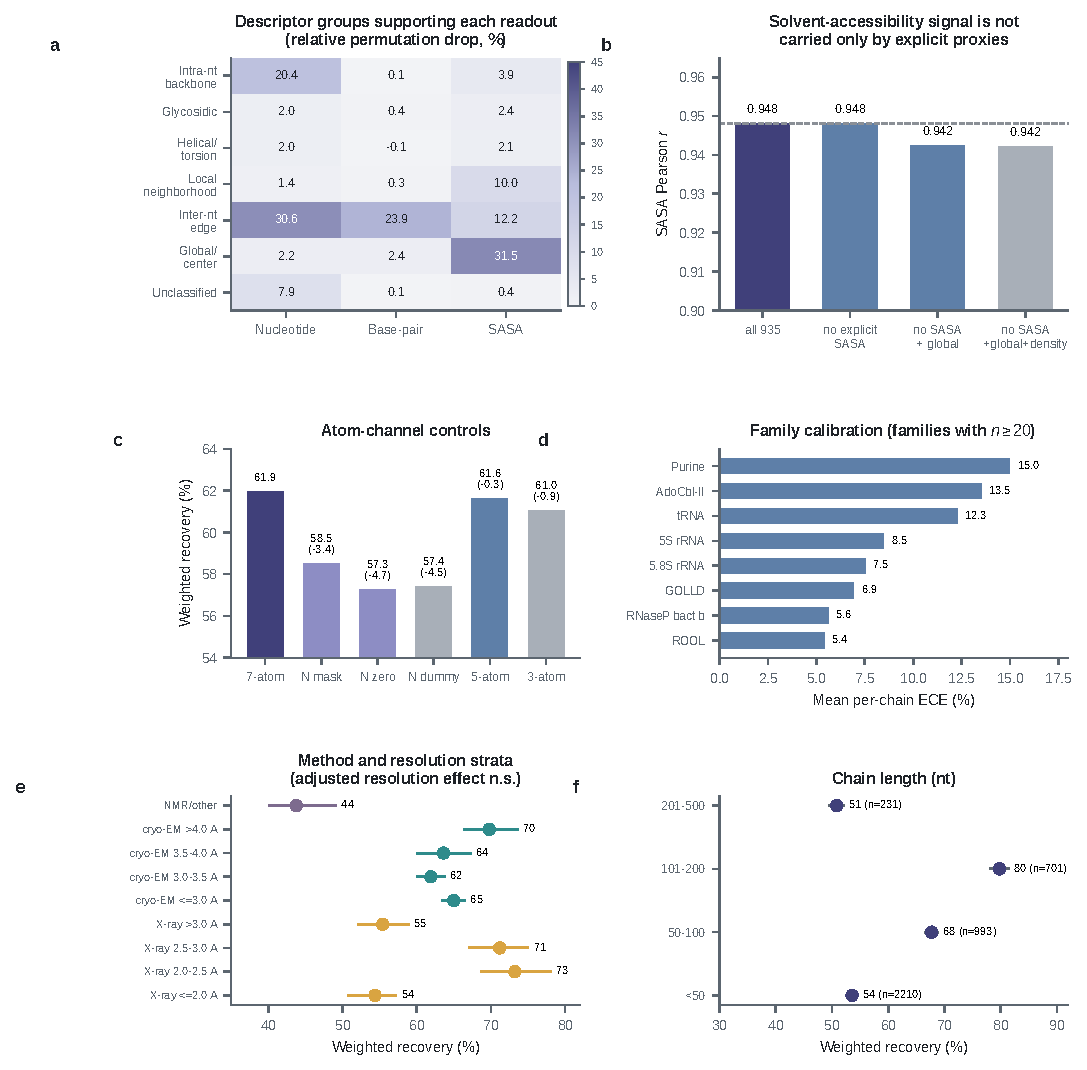
\includegraphics[width=\textwidth]{fig3_descriptors_strata.pdf}
\caption{\textbf{Complementary descriptor and stratum panels.}
\textbf{a,} Grouped permutation importance. \textbf{b,} SASA ablation. \textbf{c,}
Atom-channel controls. \textbf{d,} Family calibration (mean per-chain ECE). \textbf{e,}
Method/resolution strata. \textbf{f,} Chain-length strata. These panels support the main
information-landscape figure and are referenced where the main figure omits detail.}
\label{fig:s12_panels}
\end{figure}

\section*{Supplementary Table S13: within-puzzle OpenKnot analysis}

\begingroup\scriptsize
\begin{adjustbox}{width=\textwidth}
\begin{tabular}{lr}
\toprule
Statistic & Value \\
\midrule
Designs / puzzles & 8,125 / 21 \\
Pooled Spearman & 0.289 \\
Within-puzzle normalized rank correlation & 0.078 \\
Held-out-target Spearman, mean (range) & 0.088 ($-0.363$ to $+0.513$) \\
Leave-one-puzzle-out pooled range & 0.171--0.330 \\
Per-puzzle Spearman range & $-0.363$ to $+0.513$ \\
Held-out MFE+GC+length baseline $\rho$ & 0.316 \\
Held-out + FORGE CE $\rho$ & 0.332 \\
Held-out $\Delta\rho$, positive puzzles & $+0.016$; 13/21 \\
\bottomrule
\end{tabular}
\end{adjustbox}
\endgroup

The held-out baseline merge uses the stable key (puzzle, sequence, method, round), with
duplicate keys aggregated by mean; 8,125 scored and 8,125 MFE rows collapse to 7,837
unique keys (no many-to-many amplification). The pooled association is not evidence of
target-generalizing design ranking:
normalized within-puzzle correlation is weak, held-out-target prediction is mixed, and
leave-one-puzzle-out is a deletion sensitivity, not a held-out validation.

\section*{Supplementary Figure S14: ligand context and NMR ensemble flexibility}

\begin{figure}[htbp]
\centering
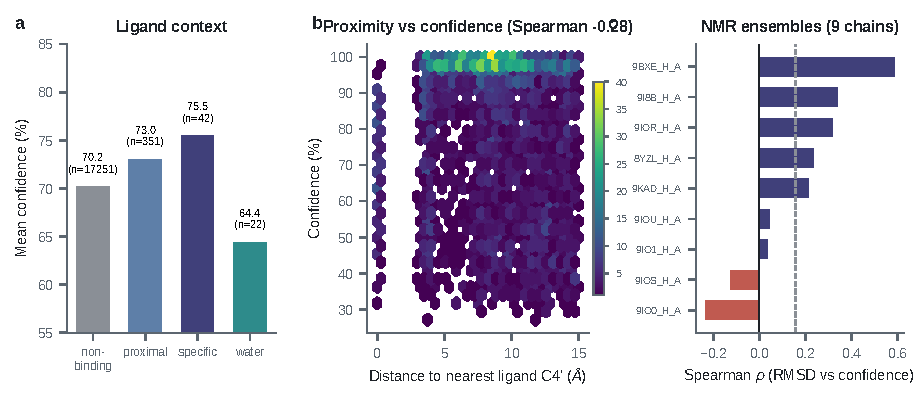
\includegraphics[width=\textwidth]{fig_s13_context.pdf}
\caption{\textbf{Context case studies.}
\textbf{a,} Mean FORGE confidence for non-binding, ligand-proximal, ligand-specific and
water-proximal positions in 200 post-2025 ligand-annotated chains. \textbf{b,} Hexbin of
minimum ligand C4$'$ distance versus confidence (Spearman $\rho=-0.28$). \textbf{c,}
Per-chain Spearman correlation between NMR ensemble mean per-residue P-atom displacement
and FORGE confidence for nine post-2025 ensembles (mean $\rho=0.16$; dashed line). Ligand analyses
are descriptive; only modelled ligands are annotated and absence of a ligand is not
evidence of non-binding.}
\label{fig:s14_context}
\end{figure}

\paragraph{Ligand-context analysis.} The 200 post-2025 chains in
\texttt{binding\_annotations\_v2.json} provide per-position ligand/ion/water distances;
we mapped annotations to residue positions, added FORGE predictions and compared mean
confidence and accuracy by binding class. Classes with fewer than five positions are not
interpreted. The analysis is descriptive and does not establish causal ligand effects. All 200 chain lengths match their FASTA; an in-range join retained 17,678 of 17,991
annotations (313 excluded as out-of-range or non-A/C/G/U). This checks position bounds
and A/C/G/U identity against the FASTA, not full residue-ID alignment.
PDB-clustered bootstrap of the specific-versus-non-binding confidence difference gave
$+0.053$ (95\% CI $-0.048$ to $+0.148$), so the ligand-class contrast is uncertain across
the 54 PDB entries.

\paragraph{Continuous stacking analysis.} For 200 post-2025 chains (13,801 unique positions) we computed an unclipped
base-plane violation for each position (centroid distance, sign-aligned normal angle and
vertical offset, normalized by the label thresholds; best neighbour retained) and
correlated it with FORGE confidence. Pooled Spearman was 0.008; the mean within-chain
Spearman was 0.060 (95\% CI 0.030--0.090); an OLS model with base and chain fixed effects
and chain-clustered errors gave a violation coefficient of $+0.041$ ($p=2.9\times10^{-13}$).
Greater geometric violation is therefore associated with slightly higher confidence;
this is not a simple stacking-order proxy or a full physical mechanism test.

\paragraph{NMR ensemble analysis.} For post-2025 NMR entries with at least two models,
per-residue P atoms present in all models were superposed by Kabsch and the mean
per-residue P-atom displacement was correlated with the cached single-structure FORGE
confidence; nine chains with at least five mapped A/C/G/U residues were retained. No
consistent confidence-flexibility relationship was observed. This is not per-conformer
inference and the residue-number mapping is not independently validated. An existing
per-conformer analysis of 25 multi-model groups gave XGBoost call consistency 0.903 and a
weak dispersion-inconsistency correlation ($r=0.084$); across 11 post-2025 ensembles,
accuracy was 0.352 in the high-dispersion half and 0.408 in the low-dispersion half. These are bounded descriptive results, not thermodynamic or dynamic measurements. A
two-ensemble per-conformer pilot (1A60, 24 models/44-residue chain; 1BYJ, 38
models/27-residue chain; 70 positions retained after requiring all backbone atoms in every
model; both pre-2025) gave accuracy 0.605, mean native-probability
s.d. 0.064 and a call-switch rate of 0.255; the high-feature-variation tertile had switch rate
0.272 and probability s.d. 0.067 versus 0.175 and 0.059 in the low-feature-variation tertile.
This is a pre-2025 pilot, not post-2025 generalization or a thermodynamic measurement.

The 9IWF Purine card remains a static single-structure illustration; no residue-level
partner-contact/error decomposition is claimed. The protein/assembly burial and
modification-ledger cases are stated boundaries, not results.

\section*{Supplementary Table S15: validation-selected confidence threshold}

\begingroup\scriptsize
\begin{adjustbox}{width=\textwidth}
\begin{tabular}{lrrr}
\toprule
Population & Threshold & Coverage & Accuracy \\
\midrule
Pre-2025 validation (selection) & 0.61 & 51.9\% & 90.1\% \\
Post-2025 all & 0.61 & 43.5\% & 88.7\% \\
Post-2025 repeats & 0.61 & 79.9\% & 95.1\% \\
Post-2025 non-repeats & 0.61 & 28.0\% & 80.8\% \\
\bottomrule
\end{tabular}
\end{adjustbox}
\endgroup

The threshold was selected on the first 1,000 pre-2025 validation chains (54,166
positions after cache/length filtering; not the full 3,293-chain split) as the smallest
0.01-grid value with at least 1,000 retained positions and at least 90\% selective
accuracy. It is applied unchanged; no post-2025 outcomes were used to choose it. PDB-clustered 95\%
CIs (1,000 bootstraps over 4,135 chains) were 40.8--46.3\% coverage and 87.8--89.4\%
accuracy for all positions, 77.9--81.7\% and 94.6--95.6\% for repeats, and 26.3--30.0\%
and 79.6--82.1\% for non-repeats. Coverage and accuracy differ substantially between
repeats and non-repeats.

\section*{Supplementary Table S16: common task contract}

\begingroup\scriptsize
\begin{adjustbox}{width=\textwidth}
\begin{tabular}{llrrl}
\toprule
Task & Evaluation unit & Chains & Positions & Baseline / note \\
\midrule
Nucleotide identity & 4-class position & 4,135 & 291,331 & random 25\%; all/repeat/joint-novel/<80\% \\
Base-pair state & binary position & 2,576 & 182,338 & majority 63.1\%; DSSR-eligible \\
Solvent exposure & continuous position & 4,135 & 291,331 & $r=0$; full-atom rSASA label \\
Reactivity target & continuous position & 4,135 & 299,074 & $r=0$; RibonanzaNet-inferred \\
Stacking & binary position & 4,135 & 290,878 & positive rate 65.7\%; exploratory \\
SS class & 3-class position & 2,138 & 163,395 & loop 54.8\%; class-balanced \\
Pseudoknot & binary rare class & 2,138 & 163,395 (11,828 positive) & prevalence 7.2\%; $F_1<0.001$ at argmax \\
\bottomrule
\end{tabular}
\end{adjustbox}
\endgroup

The common contract reports the evaluation unit, denominator, baseline and novelty
stratification where the underlying joins are valid. Auxiliary tasks remain exploratory
and are not pooled into a single benchmark score.

\section*{Supplementary Table S17: four-construct AF3 attribution matrix}

\begingroup\scriptsize
\begin{adjustbox}{width=\textwidth}
\begin{tabular}{lcccc}
\toprule
Construct & True P-RMSD (\AA) & FORGE P-RMSD (\AA) & Refined P-RMSD (\AA) & True AF3-consistent? \\
\midrule
10ZT & 6.6 & -- & -- & yes \\
10ZU & 14.1--15.8 & 22.7--23.6 & 19.5--28.2 & no (true control fails) \\
11EH & 16.2--18.6 & 25.7--27.3 & 9.4--10.5 & no (true control fails) \\
11AG & 22.1--26.9 & 18.9--22.7 & 19.1--28.2 & no (true control fails) \\
\bottomrule
\end{tabular}
\end{adjustbox}
\endgroup

Derived/refined 10ZT structures were not evaluated in this AF3 batch, so its derived rows
are left blank; SS/contact provenance is reported elsewhere (Supplementary Note S1). Three
of four true controls fail the AF3 test, so the assay cannot adjudicate designed-sequence
foldability; it only shows that FORGE/refined read-back did not yield
AF3-consistent folds in this set. \textbf{11AG interface separation.} In the two-chain 11AG stress structure, 40 residues
per chain lie within 8~\AA{} of the other chain. Interface accuracy was 30.0\% (chain A)
and 35.0\% (chain C) versus 52.5\% and 50.8\% outside the interface, while mean confidence
was similar (0.425/0.427 versus 0.432/0.438). Interface errors are therefore not explained
by lower confidence.

\section*{Supplementary Table S18: 9IWF Purine static card}

\begingroup\scriptsize
\begin{adjustbox}{width=\textwidth}
\begin{tabular}{lr}
\toprule
Quantity & Value \\
\midrule
Positions & 69 \\
Recovery & 34.8\% \\
Mean confidence & 0.476 \\
Positions with confidence $\ge 0.61$ & 1/69 \\
Accuracy, confidence 0.5--0.8 & 31.8\% (22 positions) \\
\bottomrule
\end{tabular}
\end{adjustbox}
\endgroup

A GTP ligand is present in the deposited 9IWF structure: two residues (positions 1 and
65) are within 4.5~\AA{} of GTP, with mean confidence 0.444 and accuracy 0.50 versus 0.477
and 0.343 for non-contact positions. With only two contact positions this is inconclusive,
not a contact-error mechanism. The card does not include conservation or a residue-level
decomposition into flexibility, missing chemistry, degeneracy and model failure. It is
presented as a boundary, not as a mechanism result.

\end{document}
